\chapter{Background}
This chapter covers all of the necessary background information required to
gain a well-rounded picture of basic deep learning and reinforcement learning
concepts. We briefly go through the history of the field and the chosen games,
and then move onto the technical aspects of deep learning and reinforcement
learning, such as multilayer perceptrons and Markov decision processes.

\section{History of Reinforcement Learning}

In this section, we explore the history of reinforcement learning and its
current state; this knowledge is essential for understanding the design and
implementation concepts covered later in the report.

\subsection{Operant Conditioning}
The field of reinforcement learning started in the 1970s, through B. F.
Skinner's operant conditioning \cite{skinner1971operant}. In operant
conditioning, an animal learns to associate a particular behaviour with a
reward or punishment\footnote{In reinforcement learning research, refer to
  reward and punishment as positive reward and negative reward respectively}, and
learns the researcher's desired behaviour as it is trained over time;
\autoref{fig:skinner_box} shows the device used to do this for rats. In this
case, the agent is the rat, and the actions are pressing or not pressing the
lever, with the environment being the box the rat is interacting with; it
receives rewards in the form of food. This is the basis for shaping the
behaviour of an agent, a foundational concept in reinforcement learning; we
rely on this idea as the groundwork for this project.

\begin{figure}[H]
  \centering
  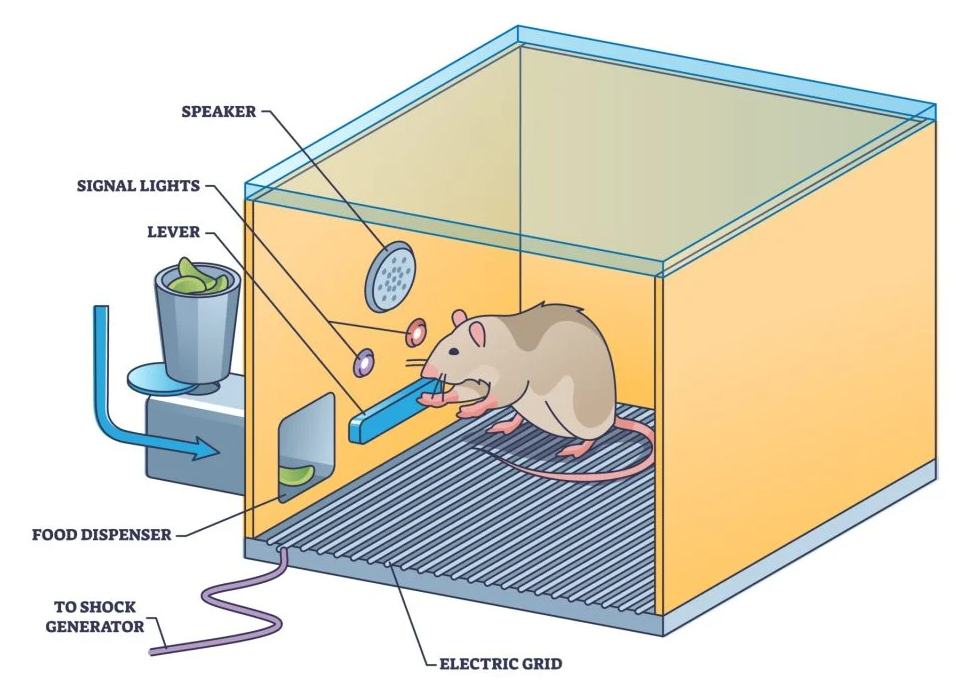
\includegraphics[width=0.5\textwidth]{figures/images/skinner_box.png}
  \caption[Skinner box]{Skinner box, used in operant conditioning experiments on rats \cite{mcleod2023b}}
  \label{fig:skinner_box}
\end{figure}


\subsection{TD Learning}
The concept of associating actions with outcomes and rewards, and
"conditioning" the agent was first applied in the context of computer science
with temporal-difference learning (TD learning), pioneered by Richard S. Sutton
in the 1980s \cite{sutton1988learning}. TD learning uses the difference between
a predicted outcome and the actual outcome of an action to update the
prediction algorithm, improving it over time. This algorithm underpins the
value based learning methods used today, including the deep Q-learning method
used in this project.

\subsection{Actor-Critic Method}
The framework for the actor-critic method was first described by Barto et al.
in 1985 as a system consisting \textit{"of a single associative search element
  (ASE) and a single adaptive critic element (ACE)"} \cite{barto1983neuronlike}.
A visual example of this method is shown in \autoref{fig:actor_critic}. This
concept lays the groundwork for the family of actor-critic methods, including
the advantage actor-critic method used in this project.

\begin{algorithm}[H]
  \caption{Tabular Actor-Critic}
  \label{alg:actor_critic}
  \begin{algorithmic}
    \State Initialize actor $\pi(a~|~s)$ with random values
    \State Initialize critic $V(s)$ with random values
    \For{episode $i$ in $1:N$}
    \State Set initial state $s_t$
    \While{$s_t$ is not terminal}
    \State Select action $a_t$ from policy $\pi(a_t~|~s_t)$ using weighted random sampling
    \State Take action $a_t$ and observe reward $r_t$ and new state $s_{t+1}$
    \State Compute TD error $\delta \gets r_t+\gamma\cdot V(s_{t+1}) - V(s_t)$
    \State Update critic values $V(s_t) \gets V(s_t) + \alpha_\text{critic}\cdot\delta$
    \State Update actor values $\pi(a_t~|~s_t) \gets \pi(a_t~|~s_t) + \alpha_\text{actor}\cdot\delta\cdot\log\pi(a_t~|~s_t)$
    \State Update state $s_t \gets s_{t+1}$
    \EndWhile
    \EndFor
  \end{algorithmic}
\end{algorithm}


\subsection{Policy Gradient Optimization}
The idea of policy gradient methods was popularized through the 1999 paper by
Sutton et al. titled "Policy Gradient Methods for Reinforcement Learning with
Function Approximation". This paper described the idea of using an
\textit{"alternative approach in which the policy is explicitly represented by
  its own function approximator"} \cite{sutton1999policy}. As the name suggests,
this method is policy based, in contrast to value based methods such as TD
learning. The idea of policy gradient optimization is what allows the actor in
the advantage actor-critic method to learn the optimal policy; we explain the
actor-critic method further in \autoref{sec:actor_critic_method_background}.

\subsection{Q-Learning}
The concept of predicting future values was later applied in the Q-learning
algorithm, proposed by Christopher Watkins in 1989 \cite{watkins1989learning}.
In Q-learning, the estimated value is the Q-value, which is the expected future
reward for each action given a state; this value is predicted using the
Q-function. An optimal policy is learned by iteratively updating this function.
A convergence proof for the algorithm was published in 1992 by Watkins and
Dayan \cite{watkins1992q}, which was generalized further in 1994 by John N.
Tsitsiklis \cite{tsitsiklis1994asynchronous}. We explore the details of
Q-learning in \autoref{sec:q_learning_background}.

\subsection{Deep Q-Learning}
Q-learning was then applied to the game of Backgammon by Tesauro et al. in
1995, producing TD Gammon \cite{tesauro1995temporal}. TD Gammon's use of neural
networks to estimate the Q-value instead of using tabular methods was a
breakthrough in reinforcement learning, as it was able to compete with and beat
expert Backgammon players. It learned complex strategies from scratch without
being explicitly programmed, which was previously unheard of.
\autoref{fig:td_gammon} shows the structure of the neural network used.

\begin{figure}[H]
  \centering
  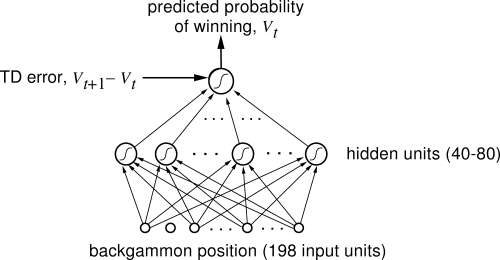
\includegraphics[width=0.7\textwidth]{figures/images/td_gammon.png}
  \caption[TD Gammon neural network]{TD Gammon neural network architecture \cite{sutton2018reinforcement}}
  \label{fig:td_gammon}
\end{figure}


Mnih et al. popularized the concept of using deep Q-networks (DQN) to play
games with their paper "Playing Atari with Deep Reinforcement Learning"
\cite{mnih2013playing}, where they achieved superhuman performance across
multiple Atari 2600 games. They later expanded the catalogue of games in 2015
\cite{mnih2015human}. We replicate the deep Q-learning strategies used in this
paper, adapting them to better suit our chosen environments.

\subsection{Asynchronous Advantage Actor-Critic}
In 2016, Mnih et al. also implemented asynchronous advantage actor-critic (A3C)
for Atari games, in their paper "Asynchronous Methods for Deep Reinforcement
Learning" \cite{mnih2016asynchronous}, vastly improving upon the performance of
the DQN. We use the concept of advantage actor-critic from this paper,
modifying it to run synchronously, as this was proven to outperform the
asynchronous version by Yuhuai Wu et al. in their 2017 paper "Scalable
trust-region method for deep reinforcement learning using Kronecker-factored
approximation" \cite{wu2017scalable}. We also make additional changes to
optimize the algorithm for Mountain Car and Car Racing.

\subsection[Recent Developments]{Recent Developments\footnote{Note the information in this section serves as context indicating the current state of the reinforcement learning space, and these concepts have not been applied directly to this project in any meaningful way}}

In 2016, a team at DeepMind developed AlphaGo to play go
\cite{silver2016mastering}, a game which was previously thought to be too
complex to be played by a program, as it has more possible board configurations
than there are atoms in the universe. AlphaGo has defeated top ranked human go
players, and, developed novel strategies after analysing expert gameplay and
using self-play to train the neural networks.

Expanding on the repertoire of games, AlphaZero was created in 2017 to master
chess, shogi and go \cite{silver2017mastering}; it achieved superhuman
performance in all three games. AlphaZero operates similarly to AlphaGo, with a
key difference being that it doesn't have access to expert gameplay; it only
uses the rule set to develop its strategies, through self-play alone.

The catalogue of games was then further expanded by MuZero in 2020, which
mastered a collection of Atari games in addition to the games played by
AlphaZero \cite{schrittwieser2020mastering}.

\begin{figure}[H]
  \centering
  \begin{subfigure}{0.26\linewidth}
    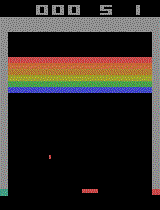
\includegraphics[height=5cm]{figures/images/breakout.png}
    \caption{Breakout}
  \end{subfigure}
  \hfill
  \begin{subfigure}{0.25\linewidth}
    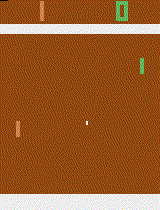
\includegraphics[height=5cm]{figures/images/pong.png}
    \caption{Pong}
  \end{subfigure}
  \hfill
  \begin{subfigure}{0.26\linewidth}
    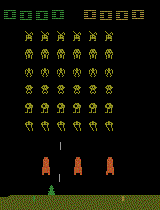
\includegraphics[height=5cm]{figures/images/space_invaders.png}
    \caption{Space Invaders}
  \end{subfigure}
  \caption[Atari games]{Popular Atari 2600 games in which AlphaZero performs with superhuman strength \cite{brockman2016gym}}
  \label{fig:atari_games}
\end{figure}


\section{Racing Games}
In this section, we briefly outline the development history of the chosen
games, and describe their mechanics as well as the reasoning for choosing these
specific games; this helps to better understand the potential improvements that
can be made to the algorithms.

Both of the racing games used in the project are well integrated into OpenAI
Gym's set of included games, alongside a larger collection of games used
commonly in reinforcement learning research \cite{brockman2016gym}.

\subsection{Mountain Car} \label{sec:mountain_car_background}
Mountain Car was first introduced by Andrew Moore in the 1990 paper "Efficient
Memory-Based Learning for Robot Control" \cite{moore1990efficient}, and was
later formalized by Satinder P. Singh and Richard S. Sutton in "Reinforcement
Learning with Replacing Eligibility Traces" \cite{singh1996reinforcement}. It
has gained popularity as a benchmark for reinforcement learning algorithms
since its introduction, and has been integrated into Gym's "Classic Control"
collection of games \cite{brockman2016gym} through which it is accessed in this
project.

The goal of Mountain Car is to reach the top of a hill, from an initial state
of the car being placed stochastically near the bottom of the hill. The car is
underpowered, meaning that an appropriate amount of force must be placed on the
car in the correct direction and from the correct position to gain momentum and
reach the yellow flag. This game has a sparse reward structure; the agent
receives a reward of -1 for each time step it takes to reach the goal, with the
episode\footnote{Episode refers to a single run of the game} ending if the
agent doesn't reach the flag within 200 time steps.

The reason for choosing Mountain Car is the simplicity of the observation and
action space; the agent receives an array containing the position and velocity
of the car, and has the option to accelerate left, do nothing or accelerate
right. This means that the game can act as a proof of concept for the
effectiveness of the chosen algorithms, and can also show the improvement
factor that domain specific enhancements provide.

\subsection{Car Racing} \label{sec:car_racing_background}
Christopher Campbell first designed Car Racing in 2014, under the name
"Top-down car" \cite{campbell2014car}. The game implements a rudimentary
physics engine to ensure the car doesn't move laterally; it contains features
such as varying surfaces that impact the car's mechanics and the ability to
drift the car, which greatly increases the difficulty of the game. Oleg Klimov
integrated the game into Gym's "Box2D" library of games \cite{brockman2016gym},
which is used by this project to access this game.

The goal of Car Racing is to complete one lap of a randomly generated track as
fast as possible, within a limited time frame. The agent is awarded -0.1 every
frame\footnote{Frame refers to a single step in the environment} and +1000/N
for every track tile visited, where N is the total number of tiles. The episode
ends if the agent doesn't complete the track within 1000 time steps or goes
outside the allowed playfield \cite{brockman2016gym}.

Contrary to Mountain Car, the reason for choosing Car Racing is the complexity
of the observation space; the agent receives a $96\times 96$ RGB image, and has
the option to do nothing, steer left, steer right, accelerate, or brake. This
combined with the complex game mechanics poses a greater challenge than
Mountain Car, and allows us to analyse the strengths and weaknesses of both
algorithms in difficult environments.

\section{Deep Learning}

Deep learning is a subset of machine learning which focuses on training
artificial neural networks on high dimensional input; this property becomes
essential in complex environments. This section discusses the techniques used
to implement the algorithms detailed in \autoref{chp:design_implementation}.

\subsection{Multilayer Perceptron}

Multilayer perceptrons (MLPs) are the foundation of artificial neural networks.
They are designed to model the neural connections in the brain, an idea first
proposed by Rosenblatt in "The Perceptron" \cite{rosenblatt1958perceptron}.

Fundamentally, an MLP is a directed graph of nodes loosely representing neurons
in the brain, which are connected to form layers. The minimum requirements for
an MLP are an input layer, at least one hidden layer, and an output layer.
These layers must be fully connected, meaning every node in one layer must be
connected to every node in the next layer. We can see an example of a simple
three layer MLP in \autoref{fig:mlp}, with two inputs, one hidden later with
three nodes, and a single output.

\begin{figure}[H]
  \centering
  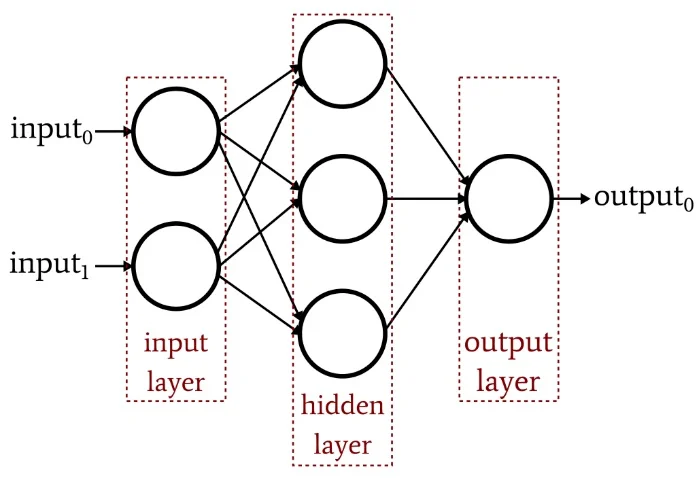
\includegraphics[width=0.5\textwidth]{figures/images/mlp.png}
  \caption[Multilayer perceptron]{Simple multilayer perceptron \cite{ledell2021statistical}}
  \label{fig:mlp}
\end{figure}


Each neuron takes the inputs $\bigl[ \begin{smallmatrix}
      x_1 \\
      \hdots \\
      x_n
    \end{smallmatrix}\bigr]$,
and computes the dot product with its stored weights
$\bigl[ \begin{smallmatrix}
      w_1 \\
      \hdots \\
      w_n
    \end{smallmatrix}\bigr]$. A bias term, $b$, is added to the result, and finally, an activation function $\phi(x)$ is applied to produce the node's output. A schematic representation of this is shown in \autoref{fig:neuron}. Different activation functions and the reasons for choosing them are explored further in \autoref{sec:activation_functions}.

\begin{gather*}
  x_{out} = \phi\left(
  \begin{bmatrix}
      x_1    \\
      \hdots \\
      x_n
    \end{bmatrix}
  \cdot
  \begin{bmatrix}
      w_1    \\
      \hdots \\
      w_n
    \end{bmatrix}
  + b\right)
\end{gather*}

\begin{figure}[H]
  \centering
  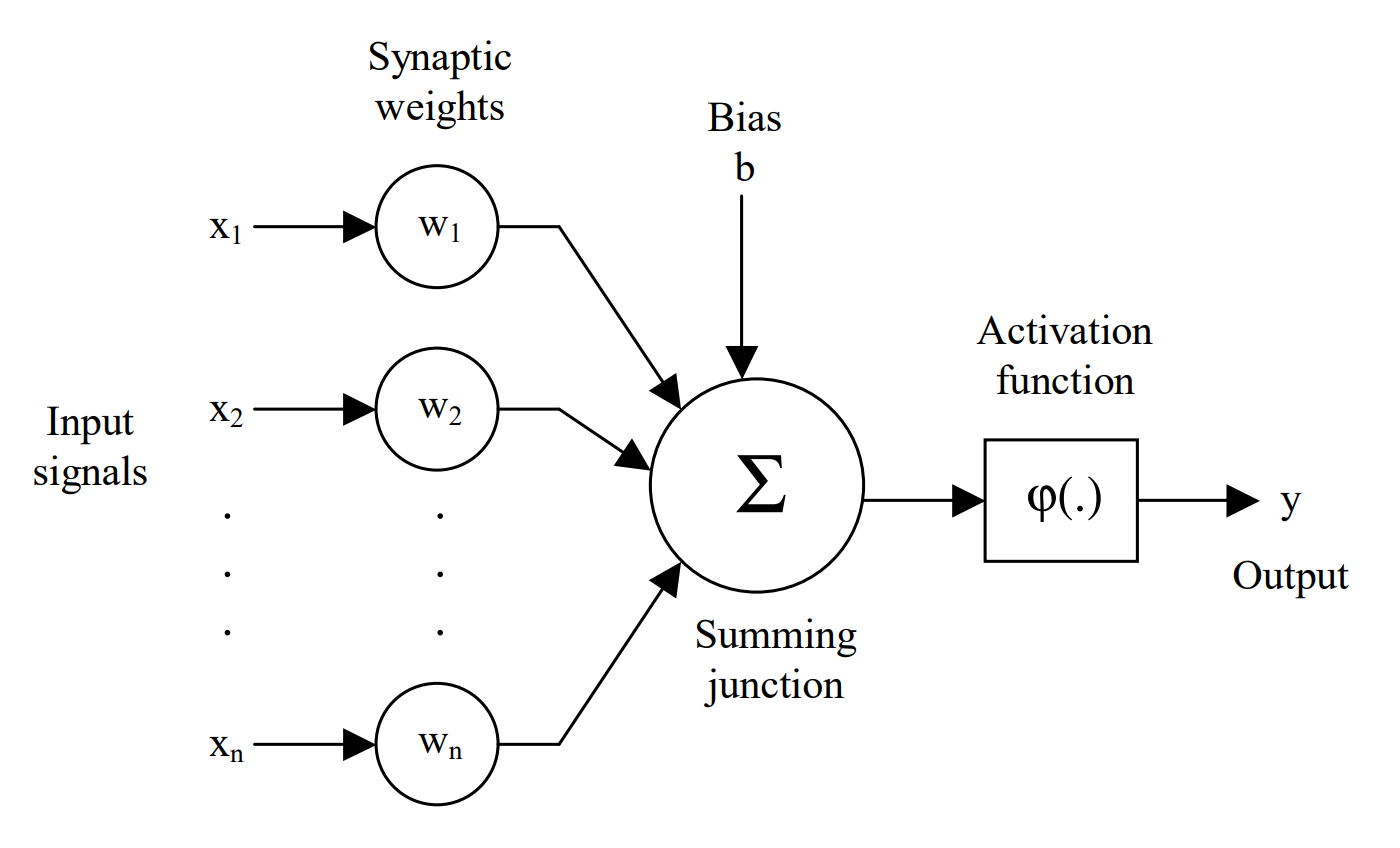
\includegraphics[width=0.7\textwidth]{figures/images/neuron.png}
  \caption[Single neuron]{Data flow and operations through single neuron \cite{csaji2001approximation}}
  \label{fig:neuron}
\end{figure}


A forward pass through the neural network is conducted layer by layer, with the
output of one layer becoming the input to the nodes in the next layer. The
final output of the MLP is the output of the last layer, which could represent
action probabilities, value estimations, etc.

Training the MLP means optimizing the weights and biases to maximize the
reward, which is done using backpropagation. This involves computing the
gradient of the reward function with respect to the weights, and using a
gradient descent method to update them, in order to reduce the difference
between the predicted output and actual output and thus improve the neural
network's prediction capabilities.

\subsubsection{Fully Connected Layers} \label{sec:connected_layers}

Due to the requirement of fully connected layers\footnote{We also refer to
  fully connected layers as "dense" layers, as this project uses Keras to
  implement the neural networks; all of the concepts are transferrable to any
  other framework}, these networks are prone to overfitting\footnote{Overfitting
  occurs when a model gives accurate predictions for the training data, but
  inaccurate predictions for unseen data} to the input and are therefore less
generalizable to novel inputs. Techniques to mitigate this issue include:

\begin{itemize}
  \item \textbf{Regularization} -- adding a penalty term (usually proportional to the weights) to the loss function, forcing the network to have sparse weights \cite{krogh1991simple}
  \item \textbf{Dropout} -- randomly "removing" neurons during training, preventing the network from relying too heavily on any one neuron \cite{srivastava2014dropout}
  \item \textbf{Batch normalization} -- normalizing the input of each layer to the neural network to have zero mean and unitary standard deviation, improving training stability and speed \cite{ioffe2015batch}
\end{itemize}

\subsubsection{Activation Functions} \label{sec:activation_functions}

The primary reason for using activation functions in MLPs is to introduce
non-linearity into the network \cite{sharma2017activation}. Without using them,
the output of a neural network can be described as a linear combination of the
input vector; activation functions allow us to model the complex non-linear
relationships between the network's inputs and outputs. Additionally,
activation functions help to introduce sparsity into the neural network, by
setting some neuron activations to zero; this can be useful in reducing
overfitting and improving the network's generalization.

Every activation function has its strengths and weaknesses. Commonly used
activation functions include:

\begin{itemize}
  \item \textbf{Rectified linear unit (ReLU)} -- returns 0 for any negative input and the input value for any positive input; often used in between convolution layers in convolutional neural networks
        $$\text{ReLU}(x) = \max(0,~x)$$
  \item \textbf{Softmax} -- maps input values to a probability distribution over the output classes, ensuring that the sum of the probabilities is equal to 1; often used in the output layer of neural networks that produce probability values
        $$\sigma(\vec{z})_i = \frac{e^{z_i}}{\sum_{j=1}^K e^{z_j}}$$
  \item \textbf{Tanh} --  maps inputs to a value between -1 and 1; often used in the fully connected hidden layers of a neural network as it can produce both positive and negative values
        $$\tanh(x) = \frac{e^x - e^{-x}}{e^x + e^{-x}}$$
\end{itemize}

We can see the graphical representation of these functions in
\autoref{fig:activation_functions}.

\begin{figure}[H]
  \centering
  \begin{subfigure}{0.27\linewidth}
    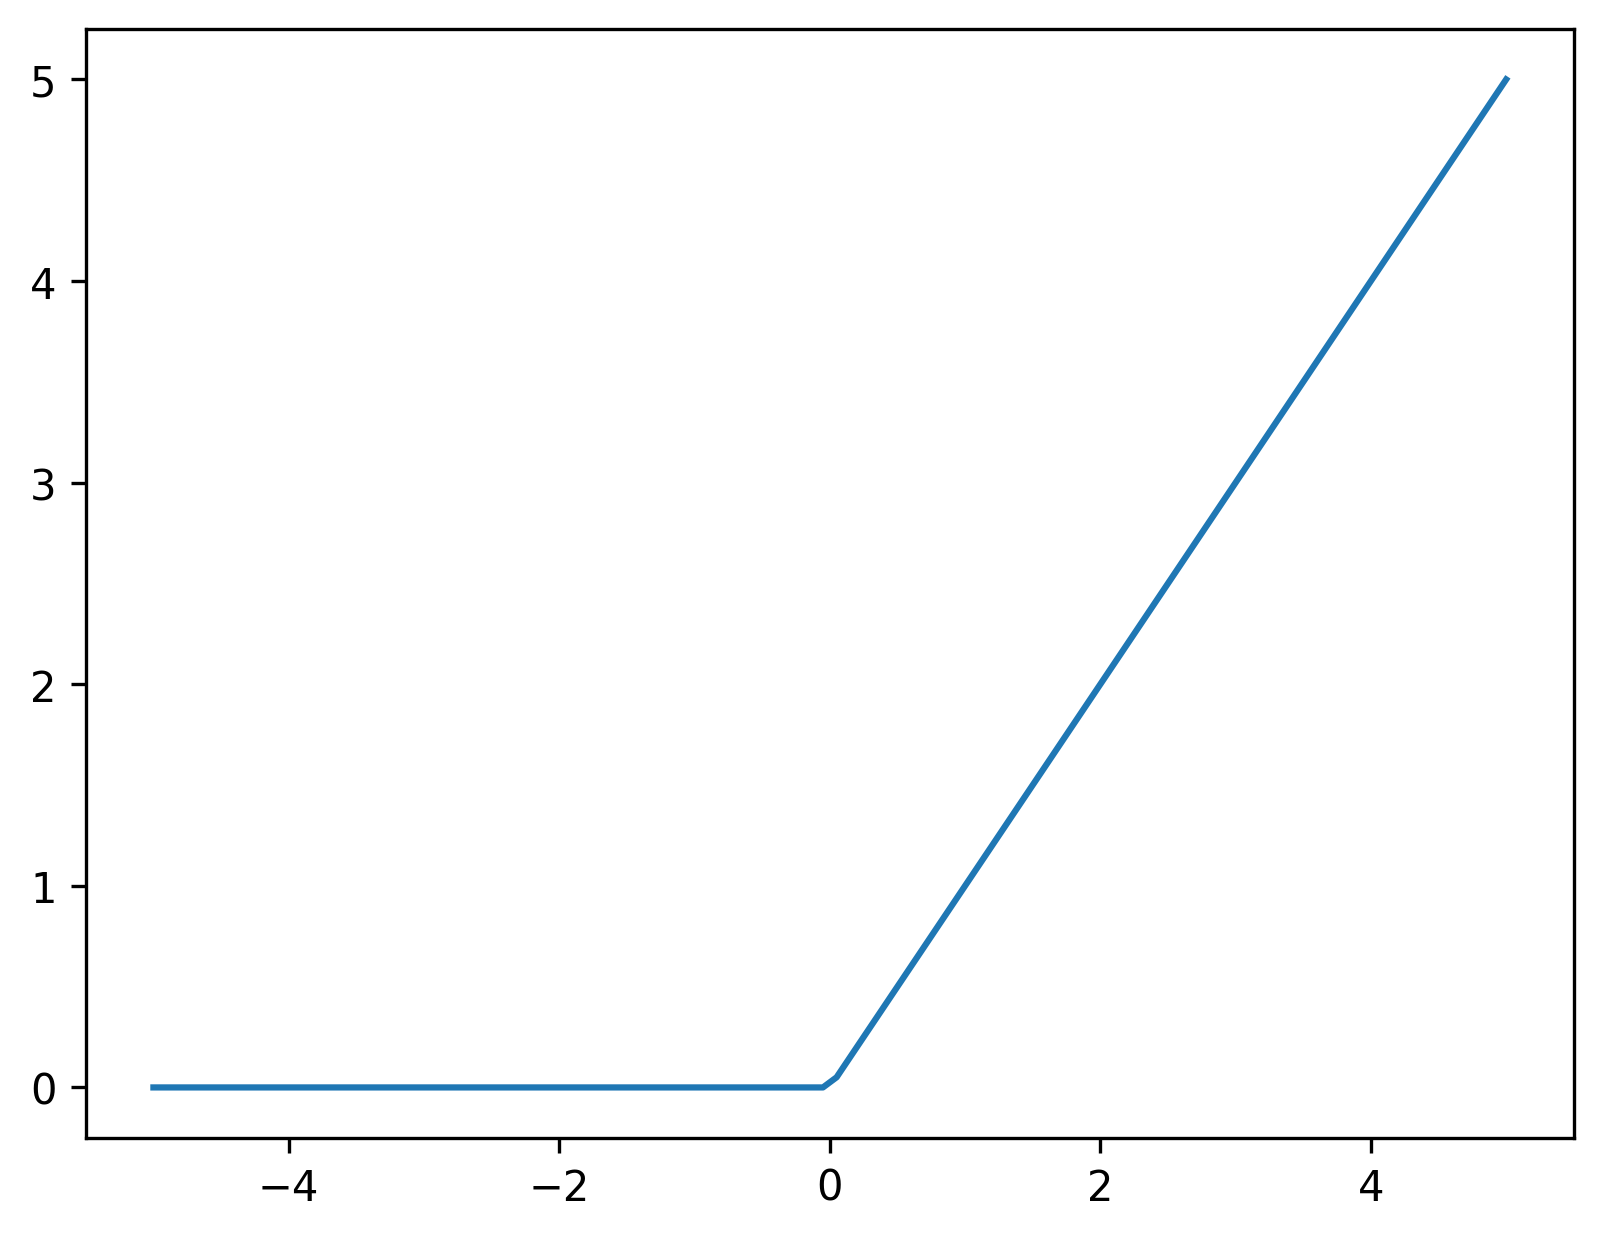
\includegraphics[height=3cm]{figures/images/relu.png}
    \caption{ReLU}
  \end{subfigure}
  \hfill
  \begin{subfigure}{0.28\linewidth}
    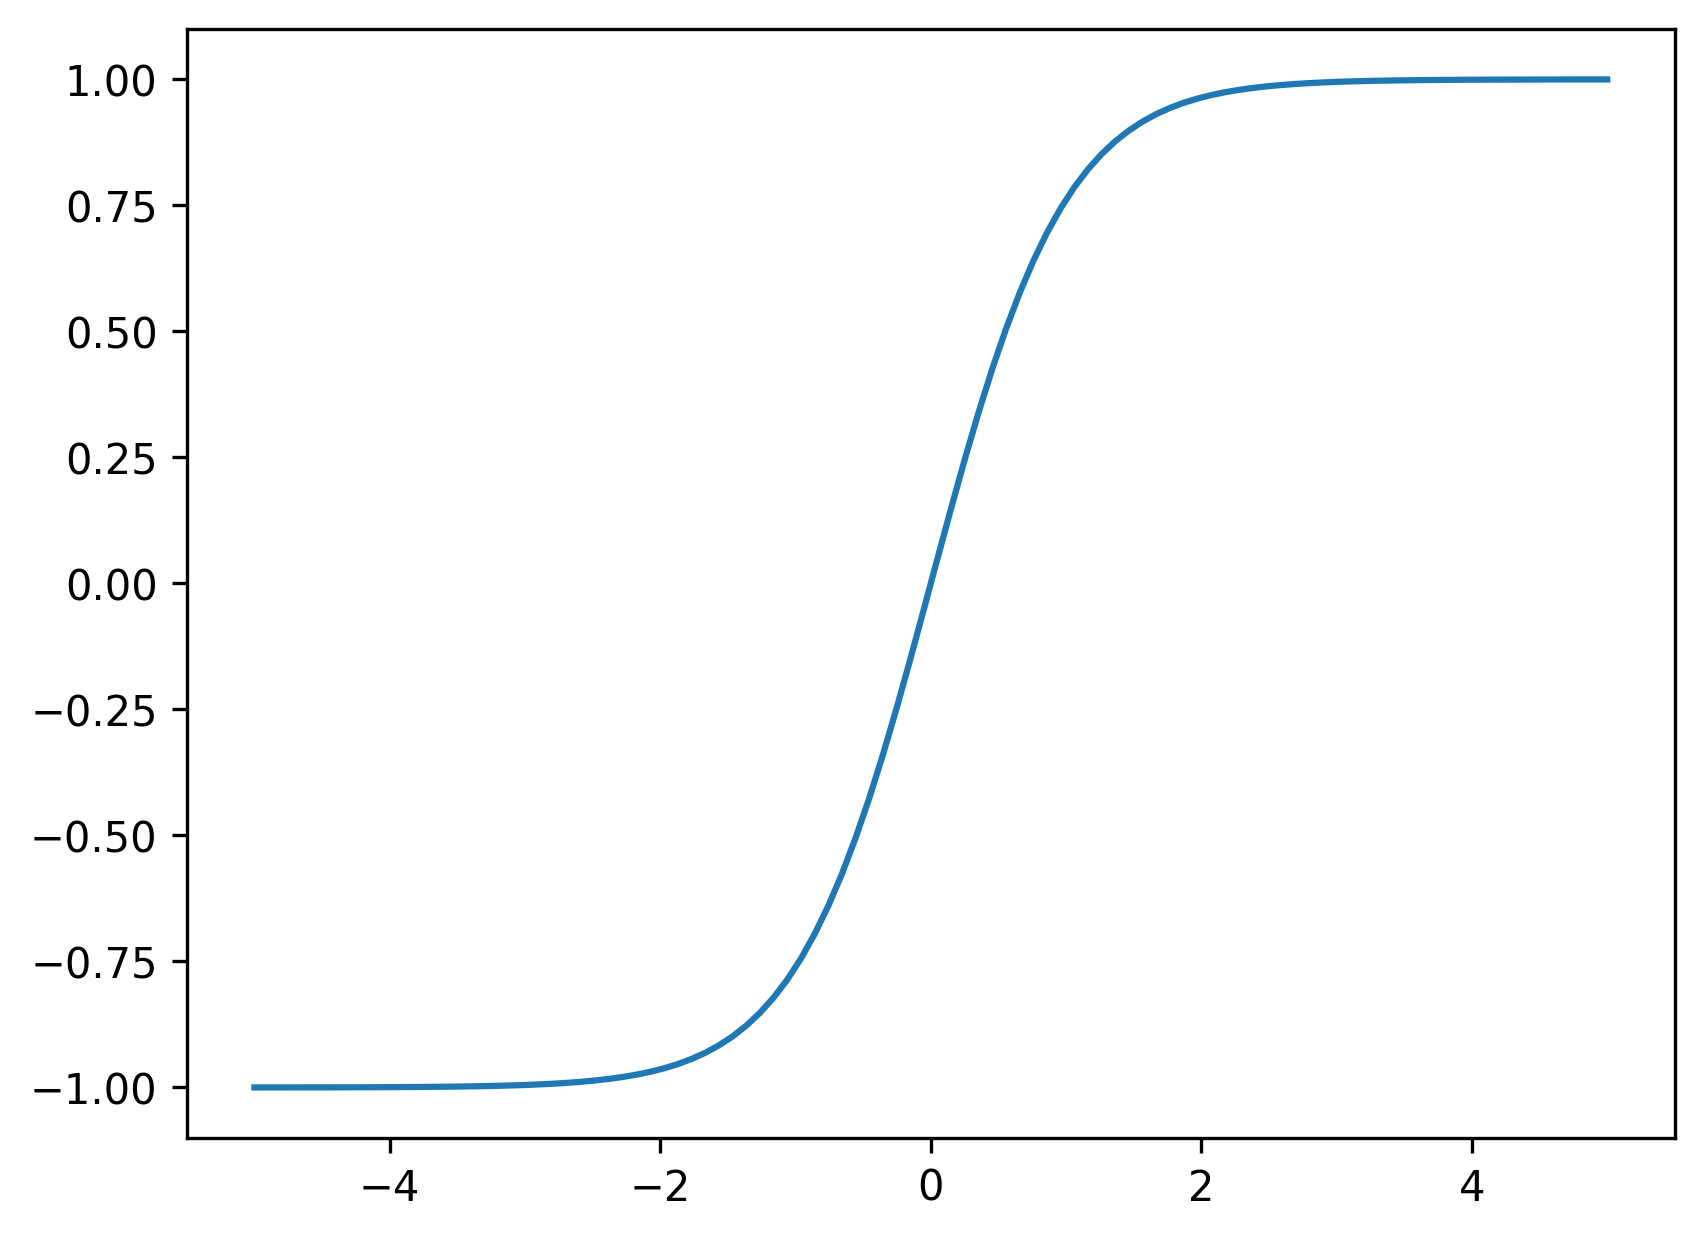
\includegraphics[height=3cm]{figures/images/tanh.png}
    \caption{Tanh}
  \end{subfigure}
  \hfill
  \begin{subfigure}{0.28\linewidth}
    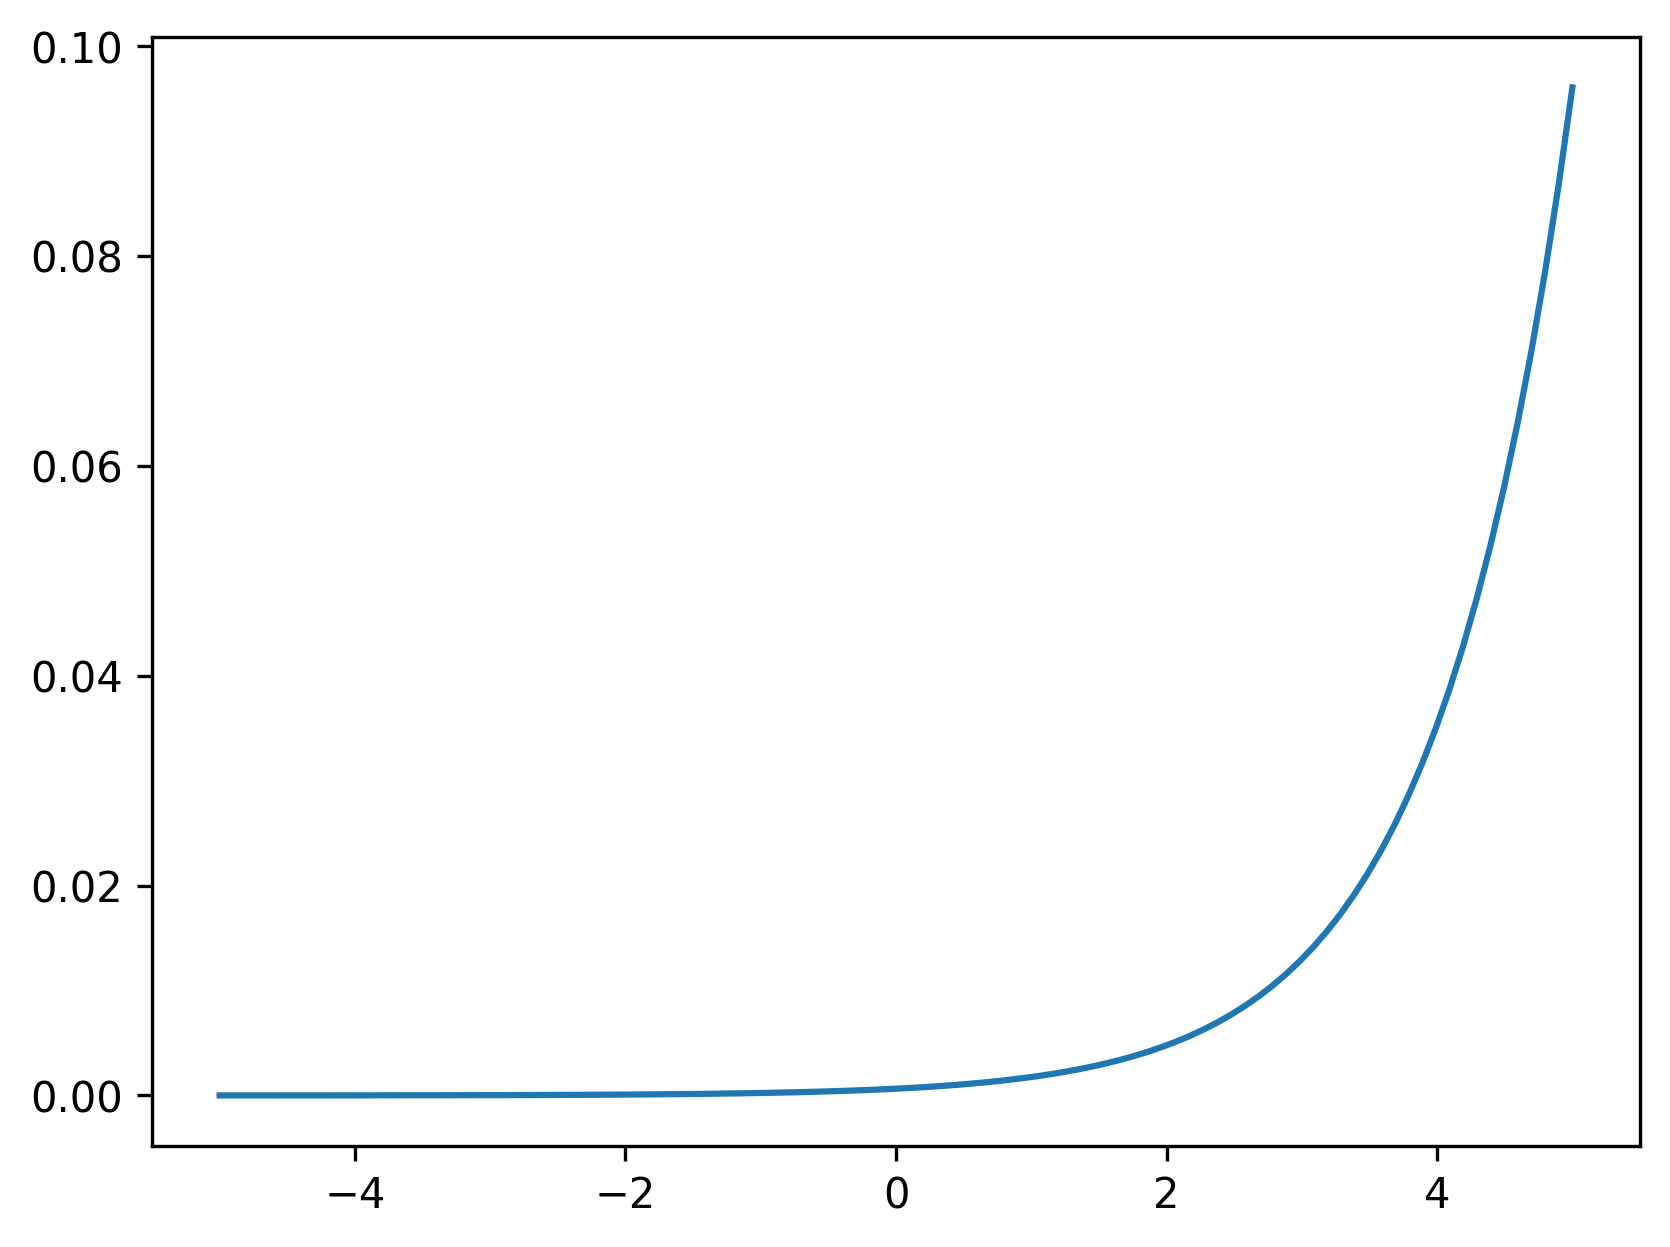
\includegraphics[height=3cm]{figures/images/softmax.png}
    \caption{Softmax}
  \end{subfigure}
  \caption[Activation functions]{Commonly used activation functions}
  \label{fig:activation_functions}
\end{figure}


\subsection{Convolutional Neural Network}

While it is possible to acquire vectorized data about the direct properties of
the environment and agent (for example, car position and velocity in Mountain
Car), this is not always the case. We often only have access to observational
image data (such as the bird's eye view in Car Racing), and we need to make
decisions based on this limited subset of information. Due to the
multidimensional nature of images, we need to extend the functionality of our
neural networks to support these types of inputs; convolutional neural networks
(CNN) provide a way for us to do this\footnote{The functionality provided by
  CNNs can technically be implemented using MLPs, though it is much more
  difficult}. These networks maintain the spatial structure of the input image
data, and can take better advantage of localized features by using
convolutional filters and pooling layers, explained further below.

\subsubsection{Filters}

The cornerstone of CNNs is the convolutional filter. It is an $n\times n$ grid
of values; the dot product is computed between the filter weights and the input
values, as shown in \autoref{fig:conv}.

\begin{figure}[H]
  \centering
  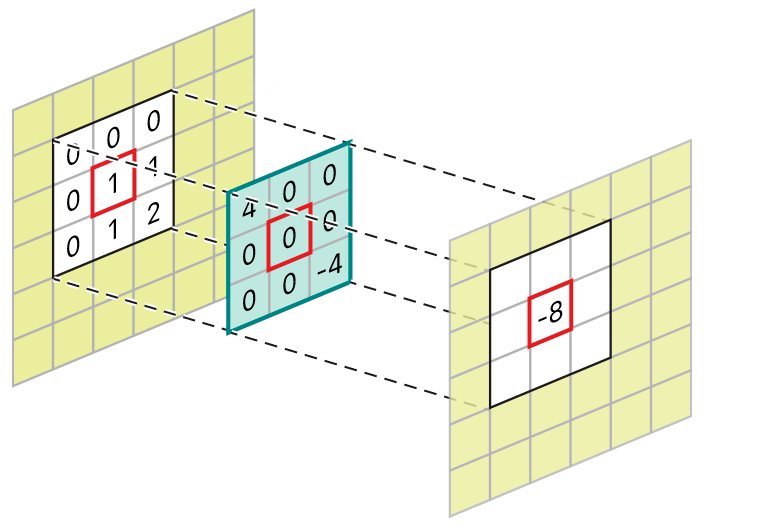
\includegraphics[width=0.5\textwidth]{figures/images/conv.png}
  \caption[Convolution filter]{Convolution filter of size $3\times 3$ being applied to an image \cite{apple0000blurring}}
  \label{fig:conv}
\end{figure}


These filters scan the input, similar to a sliding window. The step size of the
window is determined by its stride $s$, which denotes how many values to move
the filter by at each step during the convolution operation.

For each convolutional layer in a CNN, we usually have multiple filters, the
result of which is a separate layer for the output of each of the filters, as
shown in \autoref{fig:cnn}.

The weights of the filters are learnable; they are analogous to the node
connection weights in MLPs, and are optimized through gradient descent
algorithms.

\begin{figure}[H]
  \centering
  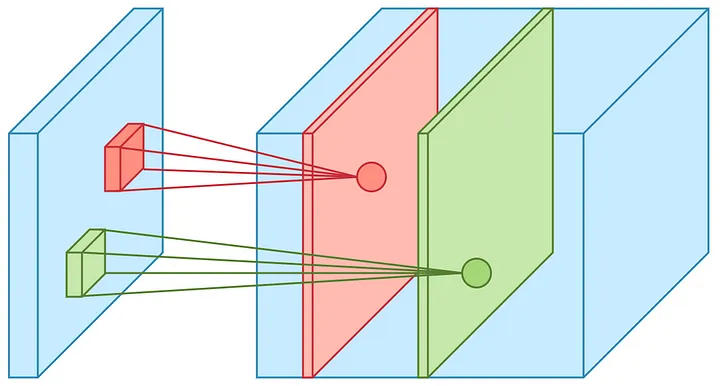
\includegraphics[width=0.5\textwidth]{figures/images/cnn.png}
  \caption[Convolutional neural network output]{Result of convolutional neural network with multiple filters applied to an input \cite{dertat2017applied}}
  \label{fig:cnn}
\end{figure}


\subsubsection{Layer Types}

The most common types of layers used in CNNs and their roles in the network are
described below:

\begin{itemize}
  \item \textbf{Convolution} -- uses a set of learnable filters to extract features and create a feature map, from either the input image or intermediary convolutional layers \cite{o2015introduction}
  \item \textbf{Pooling} -- downsamples the feature maps produced by the convolutional layers; reduces the spatial dimensions of the feature map while retaining the important information, for example max pooling, which involves taking the maximum values within specific regions of the feature map \cite{lecun2015deep}
  \item \textbf{Activation} -- applies a non-linear activation function to the output of the convolutional and pooling layers, usually ReLU
  \item \textbf{Flattening} -- converts the multidimensional output of convolutional, pooling, and activation layers into a 1D vector that can be processed by a dense layer
  \item \textbf{Dense} -- connects the output of the convolutional and pooling layers to the output layer of the network; the same as the fully connected layers in MLPs
\end{itemize}

We can see an example of the VGG16 CNN architecture in \autoref{fig:cnn_vgg},
which uses multiple sets of convolutional layers with ReLU activation and max
pooling layers, followed in the end by a series of fully connected layers. This
type of architecture is commonly used across the field of computer vision and
pattern recognition research \cite{simonyan2014very, lecun2015deep}.

\begin{figure}[H]
  \centering
  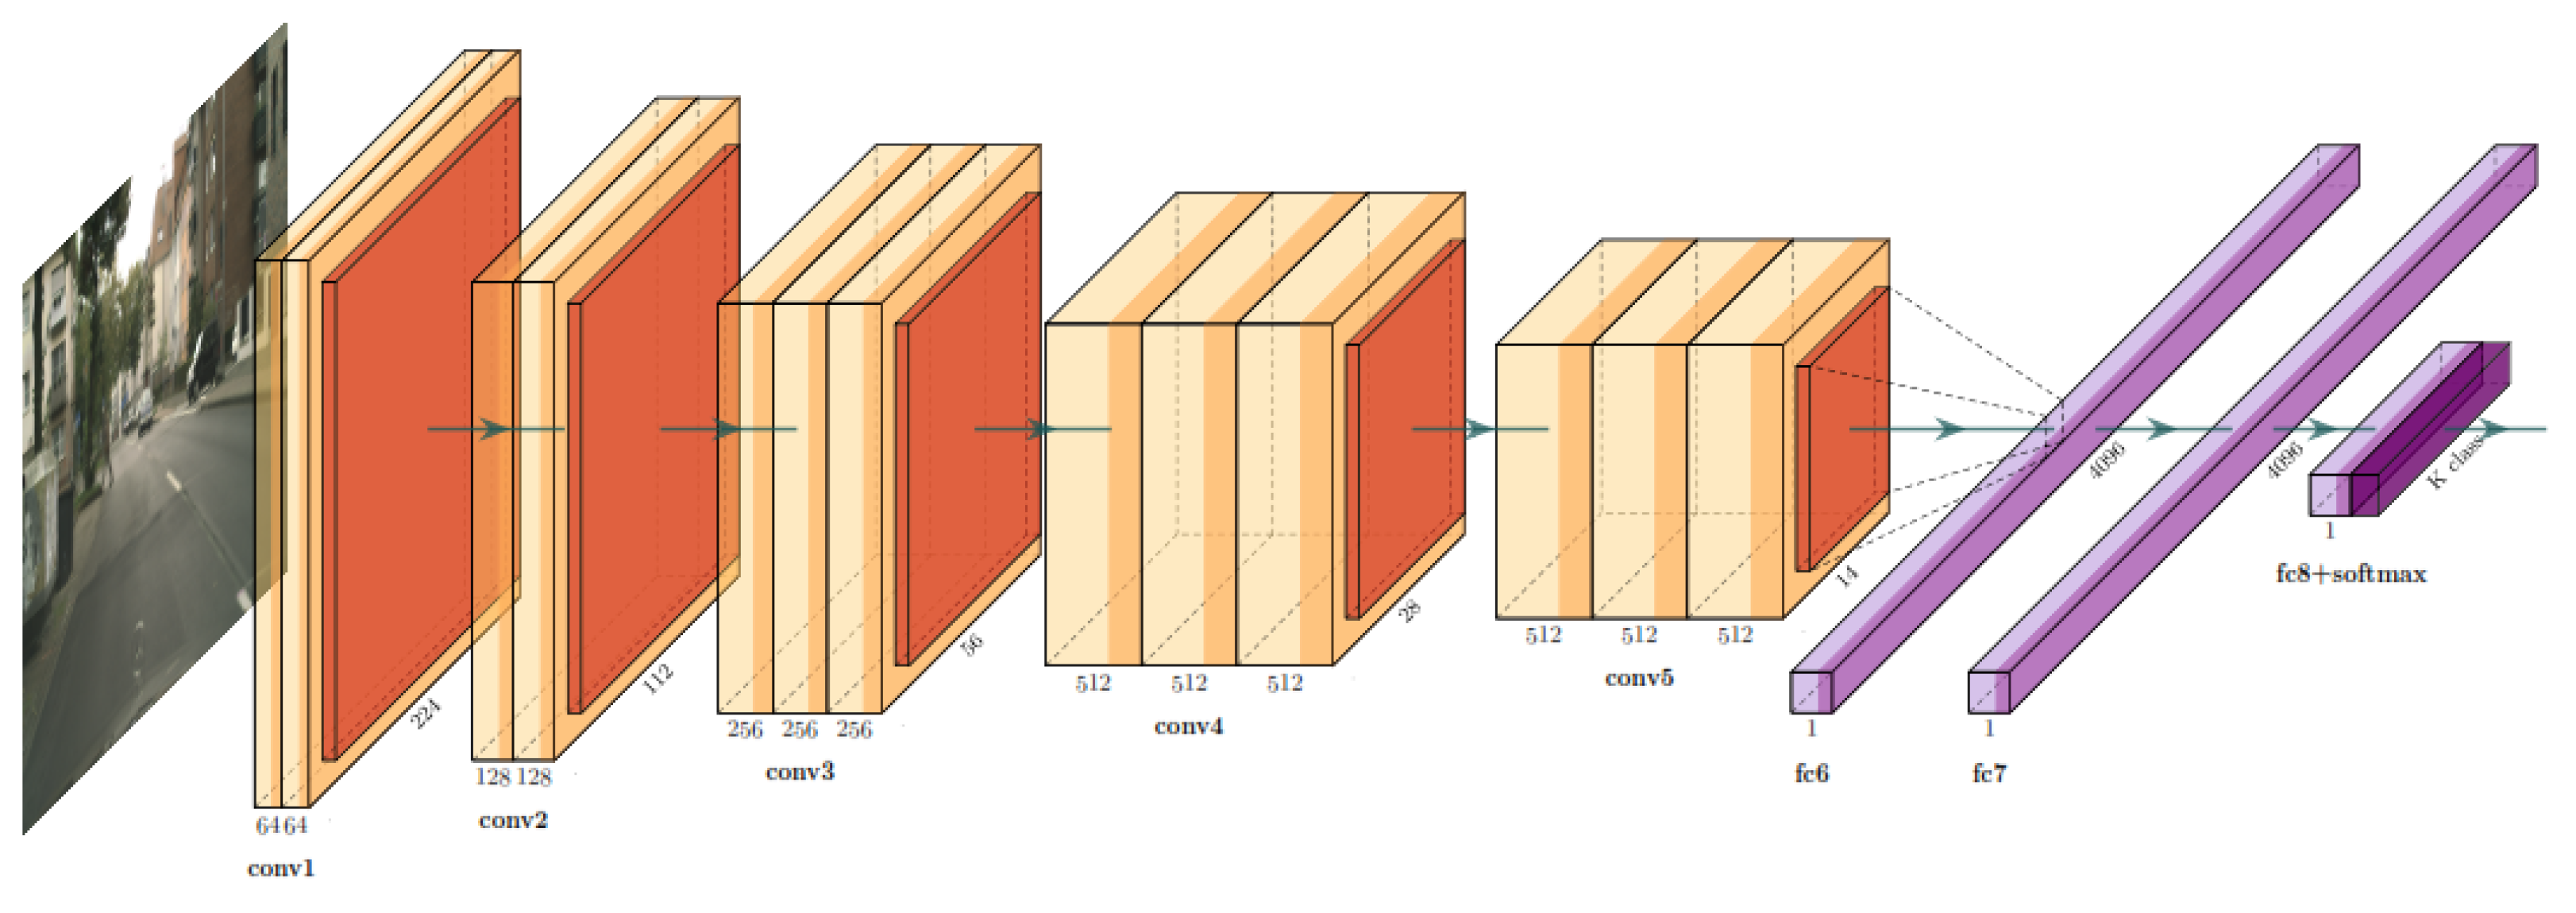
\includegraphics[width=0.9\textwidth]{figures/images/cnn_vgg.png}
  \caption[VGG16 CNN architecture]{VGG16 CNN architecture \cite{cardenas2022complex}}
  \label{fig:cnn_vgg}
\end{figure}


\newpage

\section{Reinforcement Learning} \label{sec:reinforcement_learning}

Reinforcement learning (RL) is an area of machine learning that focuses on
teaching agents to make decisions in environments, by rewarding desired
behaviours and punishing undesired ones. The goal of RL is to find the set of
actions to take in each state to maximize the cumulative reward over time,
called the policy. \autoref{fig:rl} shows the data flow through the various
components of reinforcement learning methods.

\begin{figure}[H]
  \centering
  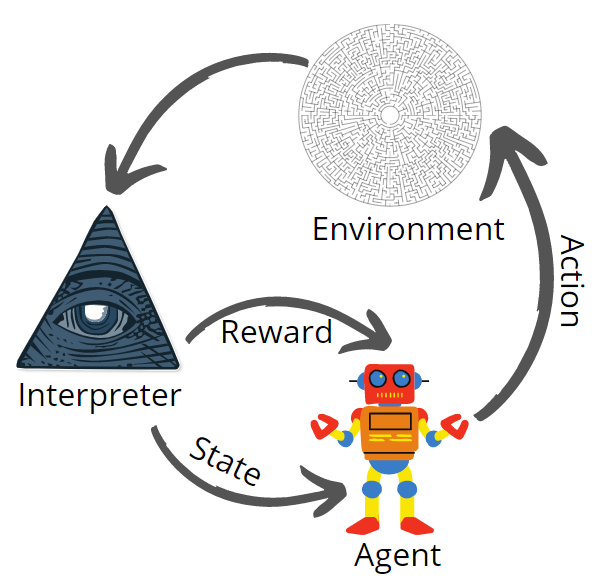
\includegraphics[width=0.4\textwidth]{figures/images/rl.png}
  \caption[Reinforcement learning flow]{Components and data flow of reinforcement learning, showing the interaction between the agent and environment; the agent takes an action based on the current state, receives a new state and a reward, and incrementally improves \cite{erainnovator2021reinforcement}}
  \label{fig:rl}
\end{figure}


The focus of this project is model-free algorithms, which means that the agent
is able to learn through trial and error by receiving and processing rewards,
without any external input. Unlike model-based algorithms, it does not rely on
an explicit model of the environment's dynamics or the reward function. The
details of model-based algorithms are not covered in this report.

\subsection{Markov Decision Process}

Markov decision processes (MDPs) are a formalization of the problem of learning
an optimal policy for an agent to take actions in an environment. The following
definitions pertaining to Markov decision processes are adapted from David
Silver's lecture series on Reinforcement Learning \cite{silver2015lecture}.

\begin{definition}
  A \textit{Markov decision process} is a tuple $\langle\mathcal{S}, \mathcal{A}, \mathcal{P}, \mathcal{R}, \gamma\rangle$
  \begin{itemize}[label={}]
    \item $\mathcal{S}$, finite set of states
    \item $\mathcal{A}$, finite set of actions
    \item $\mathcal{P}$, state transition probability matrix
          \begin{itemize}[label={}]
            \item $\mathcal{P}_{ss'}^a = \mathbb{P}~[S_{t+1}=s'\mid S_t=s,~A_t=a]$
          \end{itemize}
    \item $\mathcal{R}$, reward function
          \begin{itemize}[label={}]
            \item $\mathcal{R}_{s}^a = \mathbb{E}~[R_{t+1}\mid S_t=s,~A_t=a]$
          \end{itemize}
    \item $\gamma$, discount factor
          \begin{itemize}[label={}]
            \item $\gamma\in[0,1]$
          \end{itemize}
  \end{itemize}
\end{definition}

The state transition probability matrix $\mathcal{P}$ defines the probability
of moving from one state to another state when the agent takes a specific
action. The reward function $\mathcal{R}$ defines the immediate reward
(positive or negative) the agent receives for taking a particular action in any
given state. The discount factor $\gamma$ determines how much the system values
future rewards; $\gamma = 1$ means that future rewards are valued equally to
immediate rewards, while $\gamma = 0$ means only the immediate reward is
valued. The discount factor is a hyperparameter optimized during training, with
common values being $\gamma\in[0.95,0.99]$.

\begin{definition}
  A \textit{policy} $\pi$ is a distribution over actions given states
  $$\pi(a\mid s)=\mathbb{P}~[A_t=a\mid S_t=s]$$
\end{definition}

The policy $\pi$ is a decision-making strategy, used by the agent to determine
which action to take. It can either be a stochastic function that provides the
agent with a probability distribution over the set of possible actions for the
given state, or a deterministic function, meaning it maps the given state to a
specific action. A key feature of MDPs is that the agent's behaviour depends
only on the current state, excluding all previous states. The implications of
this are discussed in \autoref{sec:markov_property}.

\begin{definition}
  The \textit{return} $G_{t}$ is the total discounted reward from time-step $t$
  $$G_{t}=R_{t+1}+\gamma\cdot R_{t+2}+\ldots=\sum_{k=0}^{\infty}\gamma^{~k}\cdot R_{t+k+1}$$
\end{definition}

\begin{definition} \label{def:state_value_function}
  The \textit{state-value function} $v_\pi(s)$ of an MDP is the expected return starting from state $s$, and then following policy $\pi$
  $$v_\pi(s)=\mathbb{E}_{\pi}~[G_{t}\mid S_{t}= s]$$
\end{definition}

\begin{definition} \label{def:action_value_function}
  The \textit{action-value function} $q_\pi(s,~a)$ of an MDP is the expected return starting from state $s$, taking action $a$, and then following policy $\pi$
  $$q_\pi(s,~a)=\mathbb{E}_{\pi}~[G_{t}\mid S_{t}= s,~A_{t}= a]$$
\end{definition}

\begin{definition}
  The \textit{optimal state-value function} is the maximum value function over all policies
  $$v_*(s)=\max_\pi v_\pi(s)$$
\end{definition}

\begin{definition}
  The \textit{optimal action-value function} is the maximum action-value function over all policies
  $$q_*(s,~a)=\max_\pi q_\pi(s,~a)$$
\end{definition}

The goal of an MDP is to find the optimal action-value function, by finding a
policy $\pi$ that maximizes the return $G_{t}$. Once this is found, the MDP can
be considered solved, as we know which actions in any given state lead to the
highest reward.

\subsubsection{Markov Property} \label{sec:markov_property}

Simply put, the Markov property can be described as follows: the future state
of the system is independent of its past history, given its current state
\cite{markov1954theory}. We formalize this in the definition below.

\begin{definition}
  The \textit{Markov property} is a property of Markov (decision) processes
  $$\mathbb{P}~[S_{t+1}=s~|~S_t,~S_{t-1},\ldots, S_1] = \mathbb{P}~[S_{t+1}=s~|~S_t]$$
\end{definition}

This property is also known as memorylessness, because the system has no
recollection of any past states. However, this also raises the issue where the
network might not have enough information to make a decision. For example, in
\autoref{fig:car_racing_frame}, the speed of the car can not be deduced from a
single frame.

\begin{figure}[H]
  \centering
  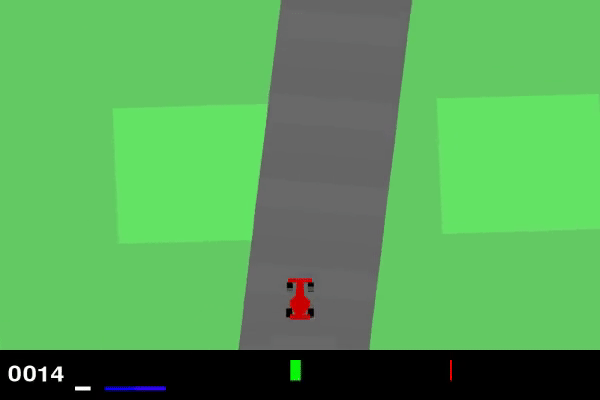
\includegraphics[width=0.5\textwidth]{figures/images/car_racing_frame.png}
  \caption[Car Racing frame]{Single frame from the Car Racing environment}
  \label{fig:car_racing_frame}
\end{figure}


To solve this, a frame stack can be used; the frame stack stores a rolling
history of states, which is then passed to the network instead of just a single
frame\footnote{A frame stack was not required for Mountain Car as the agent
  receives exact information about the car's speed and position}. This provides
the network with sufficient information to predict the optimal action. The size
of the frame stack is another hyperparameter to be optimized during training.

\subsection{Policy-Based vs Value-Based}

There are two prominent approaches to solving RL problems: policy-based
methods, and value-based methods. Hybrid methods, such as actor-critic,
incorporate components from both methods.

Policy-based methods, such as proximal policy optimization
\cite{schulman2017proximal}, focus on directly learning the policy that the
agent should follow to maximize the cumulative reward. These methods optimize
the policy using gradient descent, where the objective is to maximize the
return $G_t$. They are highly effective in continuous action space
environments, but suffer from high variance in the policy updates, leading to
learning instability.

Value-based methods, such as (deep) Q-learning, instead focus on learning the
value function, which estimates the expected cumulative reward from a given
state or state-action pair. The goal is to find the optimal state-value or
action-value function, which can be used to derive an optimal policy. Value
based methods have much more stable learning, however, they can only learn
deterministic policies.

\subsection{On-Policy vs Off-Policy} \label{sec:on_vs_off_policy}

The difference between on-policy and off-policy algorithms is whether the
behaviour policy\footnote{Behaviour policy refers to the policy used to
  determine the action to be taken in the environment} is the same as the target
policy\footnote{Target policy refers to the policy that is being "trained" in
  the neural network, which is the one we would like to optimize}. A2C is an
example of an on-policy algorithm, while DQNs are off-policy algorithms.

In an on-policy algorithm, the agent updates its target policy only using
experience generated by the same target policy. The benefit of on-policy
algorithms is that they provide more stable learning compared to off-policy
algorithms, since the same policy is used throughout the whole process.
However, it can also be less sample-efficient\footnote{Sample efficiency is the
  capability of an agent to learn with few samples}, as the collected data can
only be used once: to update the current policy.

An off-policy algorithm updates its target policy using experience generated by
a different behaviour policy. The advantage of this is that the agent can reuse
past experiences for faster learning through techniques like experience replay,
explored further in \autoref{sec:experience_replay}. However, it can also be
more challenging to stabilize the learning process, as the target policy can be
misaligned with the behaviour policy, making it a moving target.

\subsection{Exploration vs Exploitation}

The exploration-exploitation trade-off is a critical concept in RL. It
determines how the agent balances the need for exploiting the current knowledge
to maximize the reward with the need for deviating from the policy and
gathering new information for a potentially higher reward.

Too much exploration can lead to suboptimal policies and inefficient learning,
while too little exploration can lead to a lack of diversity in actions and a
failure to discover better policies. In this project, we used the
$\epsilon$-greedy approach for the DQN, and entropy regularization for the A2C
algorithm; we discuss the implementation details of these methods further in
\autoref{sec:epsilon_greedy} and \autoref{sec:entropy_regularization}
respectively.

These methods work extremely well: $\epsilon$-greedy has been shown to produce
scores better than humans \cite{mnih2013playing} in DQNs, and entropy
regularization with A2C also produces superhuman performance on similar tasks
\cite{mnih2016asynchronous}.

A few of the more advanced exploration methods include upper confidence bounds,
optimistic initialization, Boltzmann exploration, model-based exploration, and
Thompson sampling \cite{mcfarlane2018survey, ladosz2022exploration,
  gou2019dqn}; these have not been implemented in this project.

\subsection{Q-Learning} \label{sec:q_learning_background}

Q-learning is an instance of TD learning that focuses on learning an
action-value function \cite{watkins1989learning}; it is an algorithm that uses
a Q-table to store the expected future rewards, or the Q-values of taking each
action in a given state. An example of a Q-table for Mountain Car is shown in
\autoref{table:q}.

\begin{table}[H]
  \centering
  \begin{tabular}{|c|c|c|c|c|}
    \hline
    \multicolumn{2}{|c|}{\multirow{2}{*}}                    & \multicolumn{3}{c|}{\textbf{Action}}                                                      \\
    \cline{3-5}
    \multicolumn{2}{|c|}{\multirow{-2}{*}{\textbf{Q-table}}} & \textbf{Left (0)}                    & \textbf{Nothing (1)} & \textbf{Right (2)}          \\
    \hline
    \multirow{4}{*}{\textbf{State}}
                                                             & \bm{$S_0$}                           & -0.5                  & -0.2                & -0.8    \\
                                                             & \bm{$S_1$}                           & -0.1                  & -0.7                & -0.5   \\
                                                             & \textbf{\vdots}                      & \vdots               & \vdots             & \vdots \\
                                                             & \bm{$S_n$}                           & -1.0                 & -0.5                & -0.2    \\
    \hline
  \end{tabular}
  \caption[Q-table example]{Q-table showing hypothetical state-action pairs for Mountain Car}
  \label{table:q}
\end{table}


The algorithm starts with a randomly initialized table, and as the agent
interacts with the environment, it updates the table by estimating the expected
future reward for each state-action pair.

Below are the formal definitions of the Q-learning temporal difference (TD)
error and the Q-value update function.

\begin{definition} \label{def:td_error_q_learning}
  The Q-learning \textit{temporal difference (TD) error}
  $$\delta = r_t+\gamma\cdot\max_{a_{t+1}} Q(s_{t+1},~a_{t+1}) - Q(s_t,~a_t)$$
  \begin{itemize}[label={}]
    \item $r_t$, immediate reward
    \item $\gamma$, discount factor of future reward
          \begin{itemize}[label={}]
            \item $\gamma\in[0,1]$
          \end{itemize}
    \item $\max\limits_{a_{t+1}} Q(s_{t+1},~a_{t+1})$, estimate of optimal future reward for next state
    \item $Q(s_t,~a_t)$, Q-value for state-action pair
  \end{itemize}

\end{definition}

The value $r_t+\gamma\cdot\max_{a_{t+1}} Q(s_{t+1},~a_{t+1})$ is formally known
as the \textit{TD target}.

\begin{definition} \label{def:q_value_update}
  The \textit{Q-value update function}
  $$Q(s_{t},~a_{t})\leftarrow Q(s_{t},~a_{t})+\alpha\cdot\delta$$
  \begin{itemize}[label={}]
    \item $Q(s_t,~a_t)$, Q-value for state-action pair
    \item $\alpha$, learning rate
    \item $\delta$, temporal difference error
  \end{itemize}
\end{definition}

The Q-value function is semantically equivalent to the action-value function
defined previously in \autoref{def:action_value_function}.

Due to the iterative nature of this algorithm, the Q-table is updated after
each action taken by the agent. Below is the pseudocode for the Q-learning
algorithm, which demonstrates this concept.

\begin{algorithm}[H]
  \caption{Tabular Q-Learning}
  \label{alg:q_learning}
  \begin{algorithmic}
    \State Initialize Q-table $Q(s,~a)$ with random values
    \For{episode $i$ in $1:N$}
    \State Set initial state $s_t$
    \While{$s_t$ is not terminal}
    \State{
      $
        a_t =
        \begin{cases}
          \max\limits_{a_t} Q(s_t, a_t) & \text{with probability } 1-\epsilon \\
          \text{a random action }       & \text{with probability } \epsilon
        \end{cases}
      $
    }
    \State Take action $a_t$ and observe reward $r_t$ and new state $s_{t+1}$
    \State Compute TD error $\delta \gets r_t+\gamma\cdot\max\limits_{a_{t+1}} Q(s_{t+1},~a_{t+1}) - Q(s_t,~a_t)$
    \State Update Q-table values $Q(s_{t},~a_{t})\leftarrow Q(s_{t},~a_{t})+\alpha\cdot\delta$
    \State Update state $s_t \gets s_{t+1}$
    \EndWhile
    \EndFor
  \end{algorithmic}
\end{algorithm}


\subsection{Actor-Critic Method} \label{sec:actor_critic_method_background}
The actor-critic method is a hybrid reinforcement learning algorithm,
incorporating ideas from both TD learning and policy gradient methods. It
consists of two components: the actor, which decides what action the agent
takes (policy gradient), and the critic, which evaluates the quality of the
actions taken by the actor (TD learning).

Below are the formal definitions of the actor-critic temporal difference (TD)
error and both the actor and critic update functions.

\begin{definition} \label{def:td_error_actor_critic}
  The actor-critic \textit{temporal difference (TD) error}
  $$\delta = r_t+\gamma\cdot V(s_{t+1}) - V(s_t)$$
  \begin{itemize}[label={}]
    \item $r_t$, immediate reward
    \item $\gamma$, discount factor of future reward
          \begin{itemize}[label={}]
            \item $\gamma\in[0,1]$
          \end{itemize}
    \item $V(s_t)$, estimate of cumulative reward from current state
    \item $V(s_{t+1})$, estimate of cumulative reward from next state
  \end{itemize}
\end{definition}

\begin{definition} \label{def:actor_update}
  The \textit{actor update function}
  $$\pi(a_t~|~s_t) \gets \pi(a_t~|~s_t) + \alpha_\text{actor}\cdot\delta\cdot\log\pi(a_t~|~s_t)$$
  \begin{itemize}[label={}]
    \item $\pi(a_t~|~s_t)$, policy
    \item $\alpha_\text{actor}$, actor learning rate
    \item $\delta$, temporal difference error
  \end{itemize}
\end{definition}

\begin{definition} \label{def:critic_update}
  The \textit{critic update function}
  $$V(s_t) \gets V(s_t) + \alpha_\text{critic}\cdot\delta$$
  \begin{itemize}[label={}]
    \item $V(s_t)$, estimate of cumulative reward from current state
    \item $\alpha_\text{critic}$, critic learning rate
    \item $\delta$, temporal difference error
  \end{itemize}
\end{definition}

The critic is logically equivalent to the state-value function defined
previously in \autoref{def:state_value_function}. The actor and critic can be
updated either after each action, called one-step
actor-critic\footnote{One-step actor-critic is also known as episodic
  actor-critic}, or after $n$ actions, called $n$-step actor-critic
\cite{sutton2018reinforcement}. This project uses the one-step variation of the
actor-critic method, the pseudocode for which is shown below.

\begin{algorithm}[H]
  \caption{Tabular Actor-Critic}
  \label{alg:actor_critic}
  \begin{algorithmic}
    \State Initialize actor $\pi(a~|~s)$ with random values
    \State Initialize critic $V(s)$ with random values
    \For{episode $i$ in $1:N$}
    \State Set initial state $s_t$
    \While{$s_t$ is not terminal}
    \State Select action $a_t$ from policy $\pi(a_t~|~s_t)$ using weighted random sampling
    \State Take action $a_t$ and observe reward $r_t$ and new state $s_{t+1}$
    \State Compute TD error $\delta \gets r_t+\gamma\cdot V(s_{t+1}) - V(s_t)$
    \State Update critic values $V(s_t) \gets V(s_t) + \alpha_\text{critic}\cdot\delta$
    \State Update actor values $\pi(a_t~|~s_t) \gets \pi(a_t~|~s_t) + \alpha_\text{actor}\cdot\delta\cdot\log\pi(a_t~|~s_t)$
    \State Update state $s_t \gets s_{t+1}$
    \EndWhile
    \EndFor
  \end{algorithmic}
\end{algorithm}


We can observe the data flow between the different components of the
actor-critic algorithm in \autoref{fig:actor_critic_architecture}.

\begin{figure}[H]
  \centering
  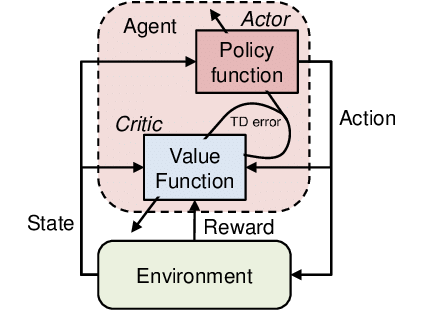
\includegraphics[width=0.5\textwidth]{figures/images/actor_critic_architecture.png}
  \caption[Actor-critic architecture]{Components and interactions in the actor-critic method \cite{fuji2018deep}}
  \label{fig:actor_critic_architecture}
\end{figure}


\section{Deep Reinforcement Learning} \label{sec:deep_rl_background}

As the name suggests, deep reinforcement learning is the combination of deep
learning and reinforcement learning. \autoref{fig:deep_rl} shows the general
architecture of a deep reinforcement learning algorithm; the agent contains a
neural network which determines the next action to be taken, and the agent
interacts with the environment receiving rewards and updating the neural
network.

\begin{figure}[H]
  \centering
  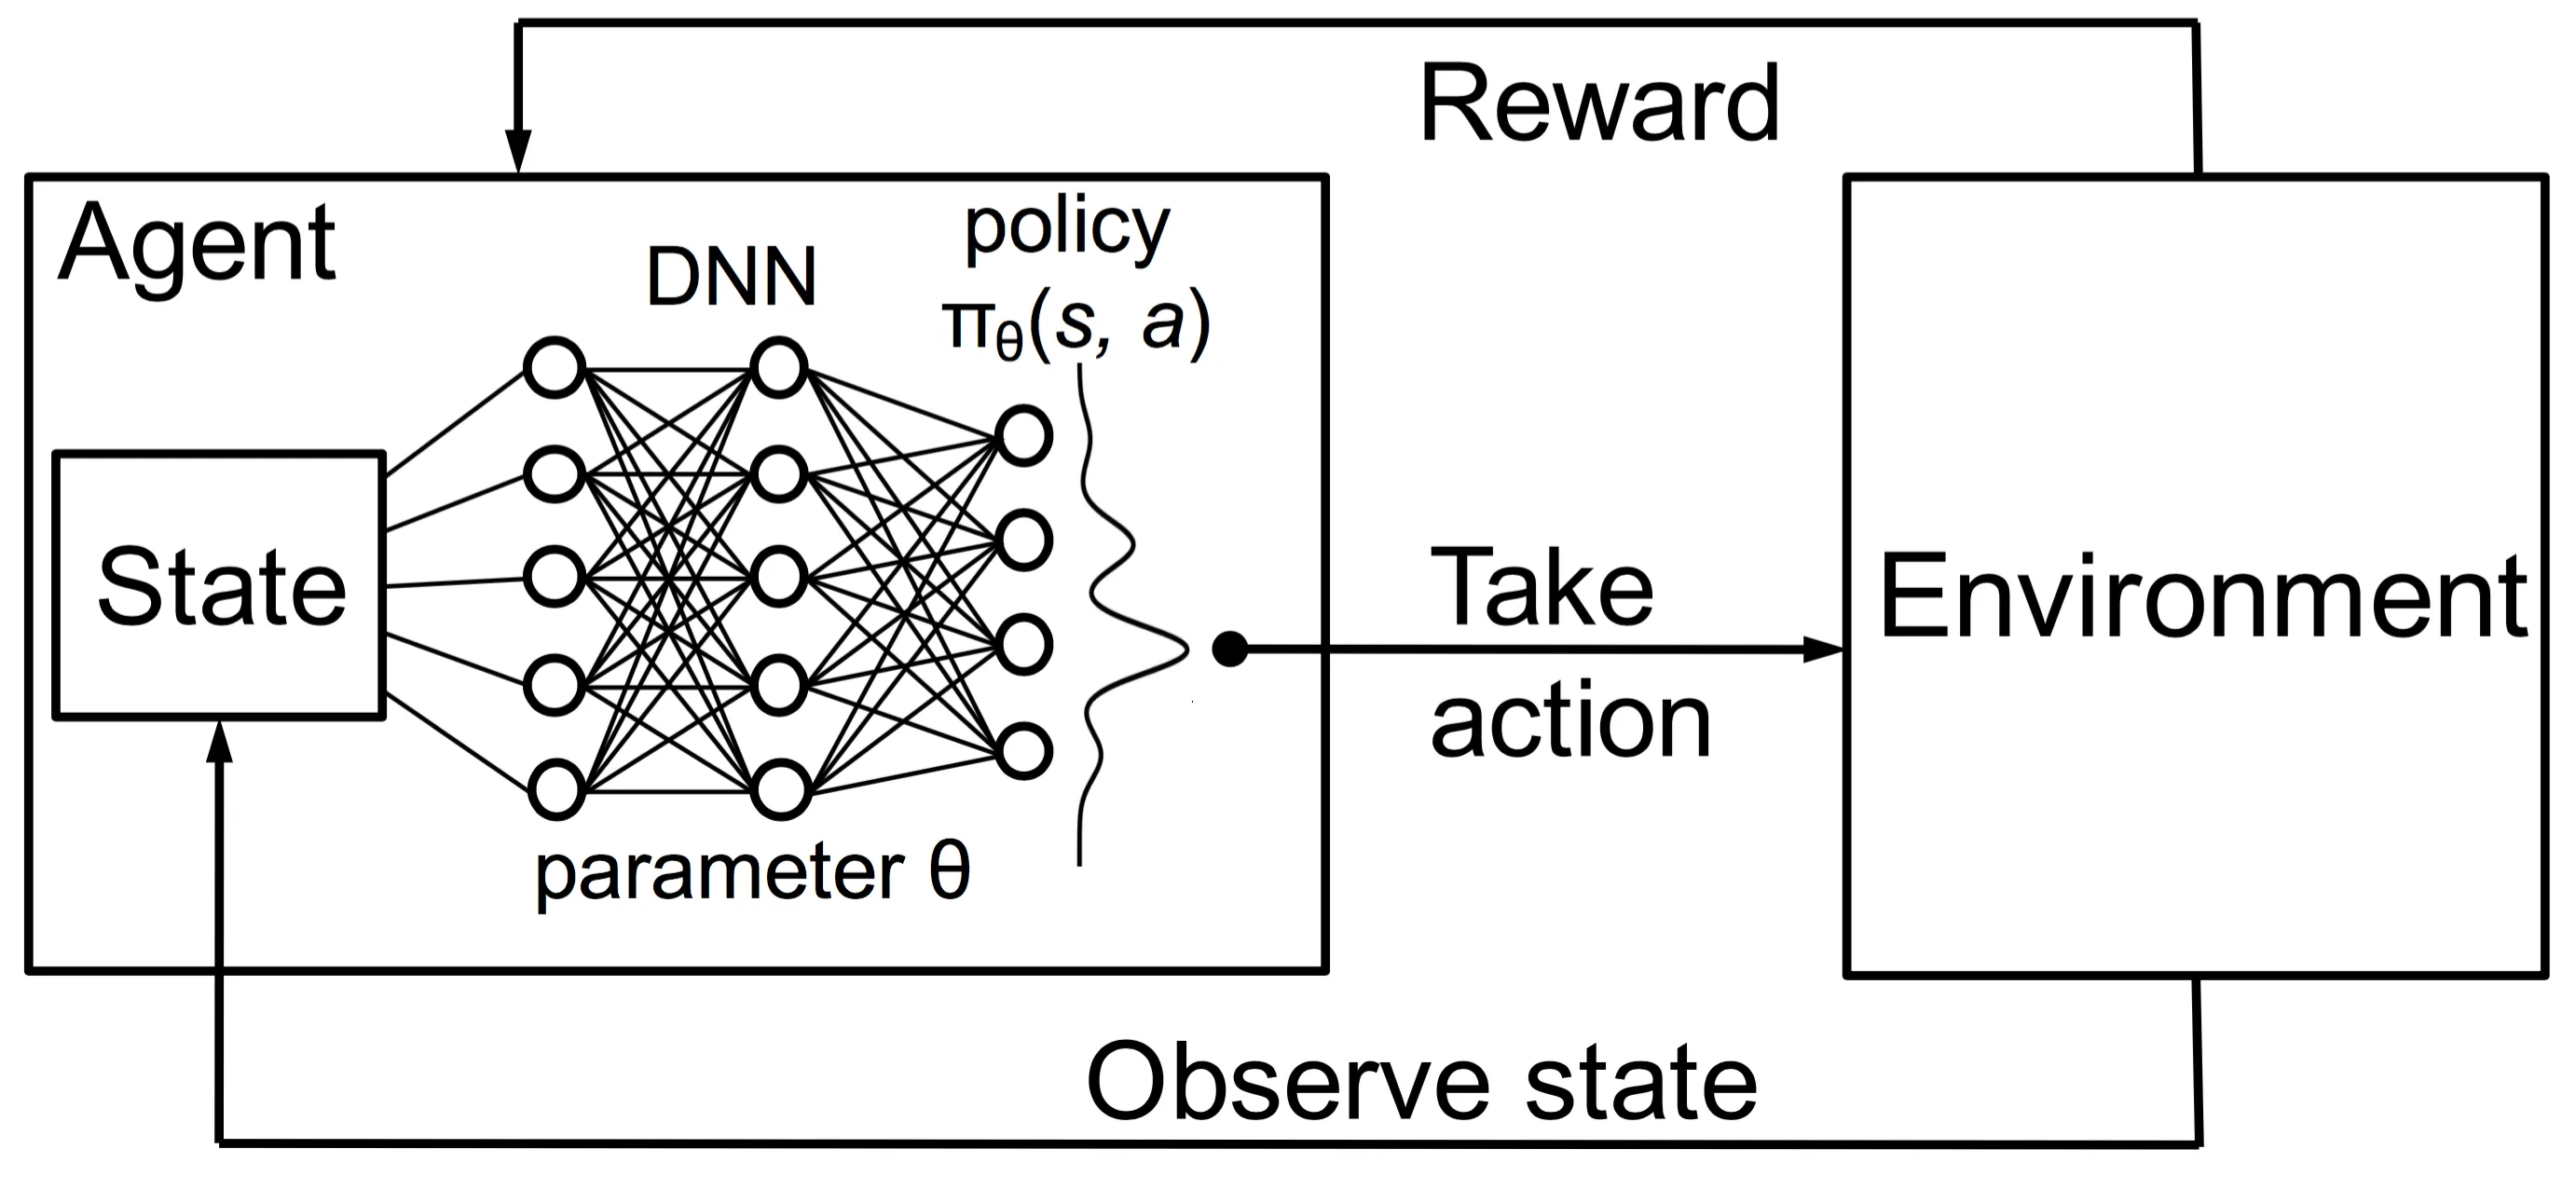
\includegraphics[width=0.6\textwidth]{figures/images/deep_rl.png}
  \caption[Deep reinforcement learning flow]{Deep reinforcement learning components and data flow, showing the interaction between the agent and environment \cite{jakhar2020reinforcement}}
  \label{fig:deep_rl}
\end{figure}


Traditional reinforcement learning methods, as described in
\autoref{sec:reinforcement_learning}, use tabular methods to approximate the
state-value or action-value function; this table becomes too large when the
observation and action space increase in size. Simple function approximators
such as linear functions can be used, although it can be very difficult to
capture the nuances of the environment using these methods.

We can overcome this obstacle with deep reinforcement learning, by instead
using a neural network to approximate the functions necessary for the chosen
algorithm; deep neural networks can handle high dimensional input, and their
size doesn't scale directly with the size of the observation and action space,
unlike tabular methods.
